\let\negmedspace\undefined
\let\negthickspace\undefined
\documentclass[journal]{IEEEtran}
\usepackage[a5paper, margin=10mm, onecolumn]{geometry}
\usepackage{lmodern} 
\usepackage{tfrupee} 
\setlength{\headheight}{1cm}
\setlength{\headsep}{0mm}   

\usepackage{gvv-book}
\usepackage{gvv}
\usepackage{cite}
\usepackage{amsmath,amssymb,amsfonts,amsthm}
\usepackage{algorithmic}
\usepackage{graphicx}
\usepackage{textcomp}
\usepackage{xcolor}
\usepackage{txfonts}
\usepackage{listings}
\usepackage{enumitem}
\usepackage{mathtools}
\usepackage{gensymb}
\usepackage{comment}
\usepackage[breaklinks=true]{hyperref}
\usepackage{tkz-euclide} 
\usepackage{listings}                             
\def\inputGnumericTable{}                                 
\usepackage[latin1]{inputenc}                                
\usepackage{color}                                            
\usepackage{array}                                            
\usepackage{longtable}                                       
\usepackage{calc}                                             
\usepackage{multirow}                                         
\usepackage{hhline}                                           
\usepackage{ifthen}                                           
\usepackage{lscape}
\usepackage{xparse}

\bibliographystyle{IEEEtran}

\title{4.3.53}
\author{EE25BTECH11062 - Vivek K Kumar}

\begin{document}
\maketitle

\renewcommand{\thefigure}{\theenumi}
\renewcommand{\thetable}{\theenumi}

\numberwithin{equation}{enumi}
\numberwithin{figure}{enumi} 

\textbf{Question}:\\
The Fahrenheit temperature $F$ and absolute temperature $K$ satisfy a linear equation.
Given that $K = 273$ when $F = 32$ and that $K = 373$ when $F = 212$. Express K in
terms of $F$ and find the value of $F$, when $K = 0$.

\textbf{Solution: }

\begin{table}[H]    
  \centering
  \begin{tabular}{|c|c|}
\hline
\textbf{Name} & \textbf{Value} \\ \hline
$\vec{A}$ & $\myvec{2 & 1 \\0 & 3}$ \\ \hline
\end{tabular}

  \caption{Variables used}
  \label{tab:4.3.53}
\end{table}

Since there is a linear relation, the equation of the straight line can be expressed as
\begin{align}
    \vec{n}^\top\vec{x} &= c\\
    \vec{A}^\top \vec{n} &= c\\
    \vec{B}^\top \vec{n} &= c\\
    \myvec{\vec{A} & \vec{B}}^\top \vec{n} &= c\myvec{1 \\ 1}\\
    \myvec{273 & 32 \\ 373 & 212} \vec{n} &= c\myvec{1 \\ 1} 
\end{align}
As $\rank\myvec{\vec{A} & \vec{B}}^\top \neq 1$ from above equation, $c \neq 0$. \\Taking $c = 1$,
\begin{align}
    \myvec{273 & 32 \\ 373 & 212} \vec{n} = \myvec{1 \\ 1} \\
    \implies \myaugvec{2}{273 & 32 & 1 \\ 373 & 212 & 1} \xleftrightarrow[]{R_2 \leftarrow R_2 - 373/273R_1} \myaugvec{2}{273 & 32 & 1 \\ 0 & 45940/273 & -100/273}\\
    \xleftrightarrow[]{R_1 \leftarrow R_1 - 8736/45940 R_2} \myaugvec{2}{273 & 0 & 2457/2297\\0 & 45940/273 & -100/273} \\
    \vec{n} = \frac{1}{2297}\myvec{9 \\ -5}
\end{align}
Substituting in line equation
\begin{align}
     \vec{n}^\top\vec{x} &= 1\\
     \myvec{9 & -5}\myvec{K \\ F} &= 2297 
\end{align}

Solving for point $\vec{C}$, $\myvec{0 \\ F}$\\
We have,
\begin{align}
    \myvec{9 & -5}\myvec{0 \\ F} = 2297\\
    F = -\frac{2297}{5}
\end{align}

\begin{figure}[H]
   \centering
  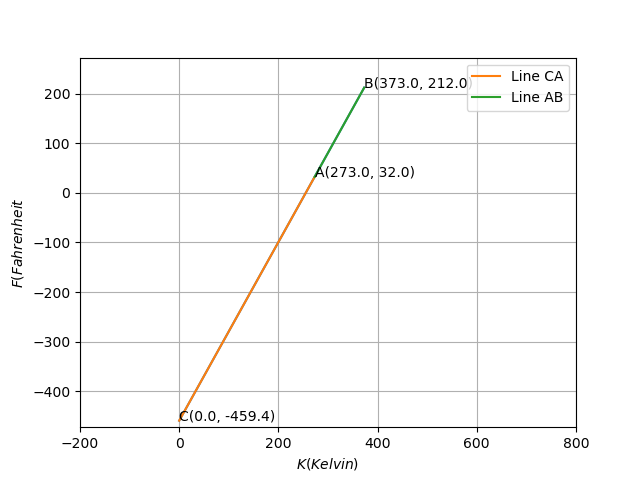
\includegraphics[width=0.64\columnwidth]{figs/fig.png}
   \caption{Given points on a line}
   \label{stemplot}
\end{figure}
\end{document}  